\section{Auswertung}

\begin{table}[H]
    \caption{Distanzmessungen bei Inkrementieren der Drehfrequenz}
    \begin{subtable}{.5\linewidth}
        \centering
        \caption{Messung von Alex Murray}
        \begin{tabular}{cc}
            \toprule
            Drehfrequenz ($Hz$) & Distanz ($\mu m$) \\
            \midrule
            498  & 0    \\
            605  & -83  \\
            702  & -169 \\
            800  & -250 \\
            885  & -324 \\
            1008 & -414 \\
            1096 & -499 \\
            1200 & -586 \\
            1305 & -666 \\
            1400 & -741 \\
            1498 & -839 \\
            \bottomrule
        \end{tabular}
    \end{subtable}
    \begin{subtable}{.5\linewidth}
        \centering
        \caption{Messung von Yohannes Measho}
        \begin{tabular}{cc}
            \toprule
            Drehfrequenz ($Hz$) & Distanz ($\mu m$) \\
            \midrule
            1498 & 0   \\
            1388 & 124 \\
            1289 & 192 \\
            1199 & 280 \\
            1106 & 353 \\
            1009 & 431 \\
            912  & 516 \\
            807  & 590 \\
            708  & 682 \\
            603  & 771 \\
            502  & 851 \\
            \bottomrule
        \end{tabular}
    \end{subtable}
\end{table}

\begin{table}[H]
    \caption{}
    \begin{subtable}{.5\linewidth}
        \centering
        \caption{Messung von Alex Murray}
        \begin{tabular}{ccc}
            \toprule
            $x (mm)$ & \hspace{5mm} & $z (mm)$ \\
            \midrule
            10.042 && 12.5 \\
            8.031  && 13.0 \\
            6.049  && 13.5 \\
            4.049  && 14.0 \\
            1.990  && 14.5 \\
            -0.019 && 15.0 \\
            -1.988 && 15.5 \\
            -3.955 && 16.0 \\
            -5.954 && 16.5 \\
            -7.973 && 16.5 \\
            -9.952 && 17.5 \\
            \bottomrule
        \end{tabular}
    \end{subtable}%
    \begin{subtable}{.5\linewidth}
        \centering
        \caption{Messung von Yohannes Measho}
        \begin{tabular}{ccc}
            \toprule
            $x (mm)$ & \hspace{5mm} & $z (mm)$ \\
            \midrule
            10.047 && 12.5 \\
            8.020  && 13.0 \\
            5.980  && 13.5 \\
            3.990  && 14.0 \\
            1.926  && 14.5 \\
            -0.053 && 15.0 \\
            -2.048 && 15.5 \\
            -4.030 && 16.0 \\
            -6.039 && 16.5 \\
            -7.997 && 17.0 \\
            -9.987 && 17.5 \\
           \bottomrule
        \end{tabular}
    \end{subtable}
\end{table}


\subsection{Messergebnisse}

\begin{figure}[H]
    \center
    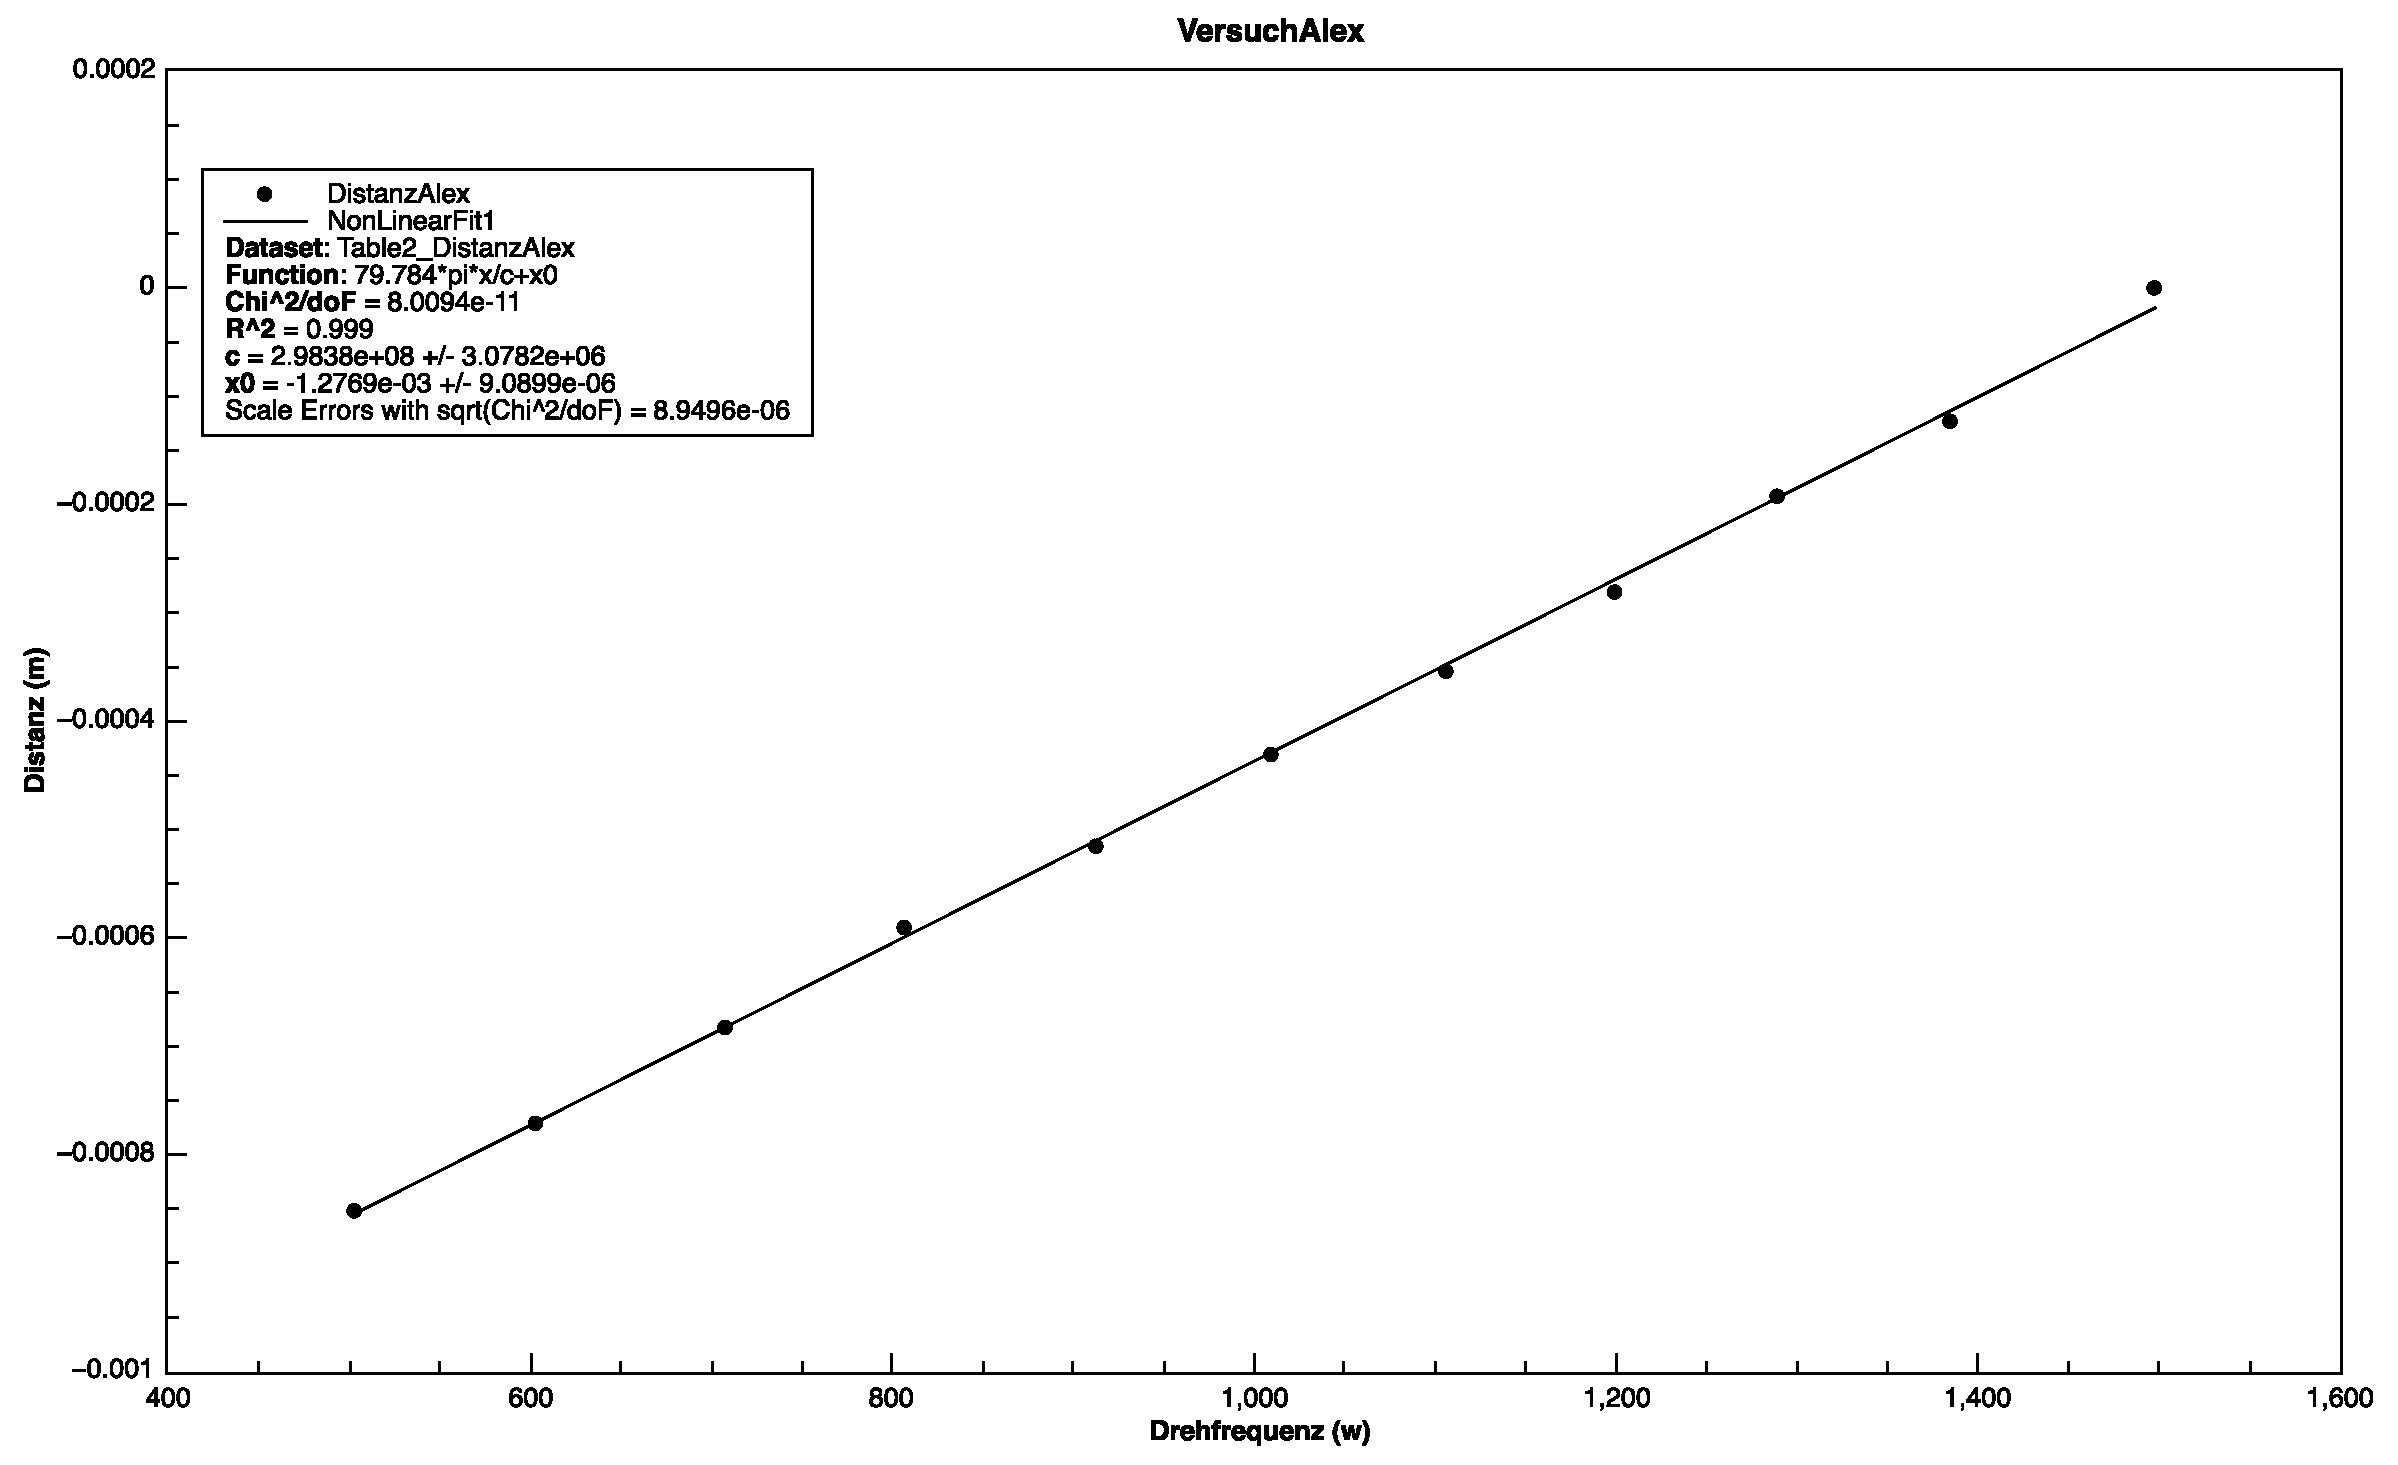
\includegraphics[width=.8\textwidth]{images/w-x-alex.pdf}
    \caption{XY-Scatter Plot von $\omega$ und $x$, gemessen von Alex Murray}
    \label{fig:w-x-alex}
\end{figure}

\begin{figure}[H]
    \center
    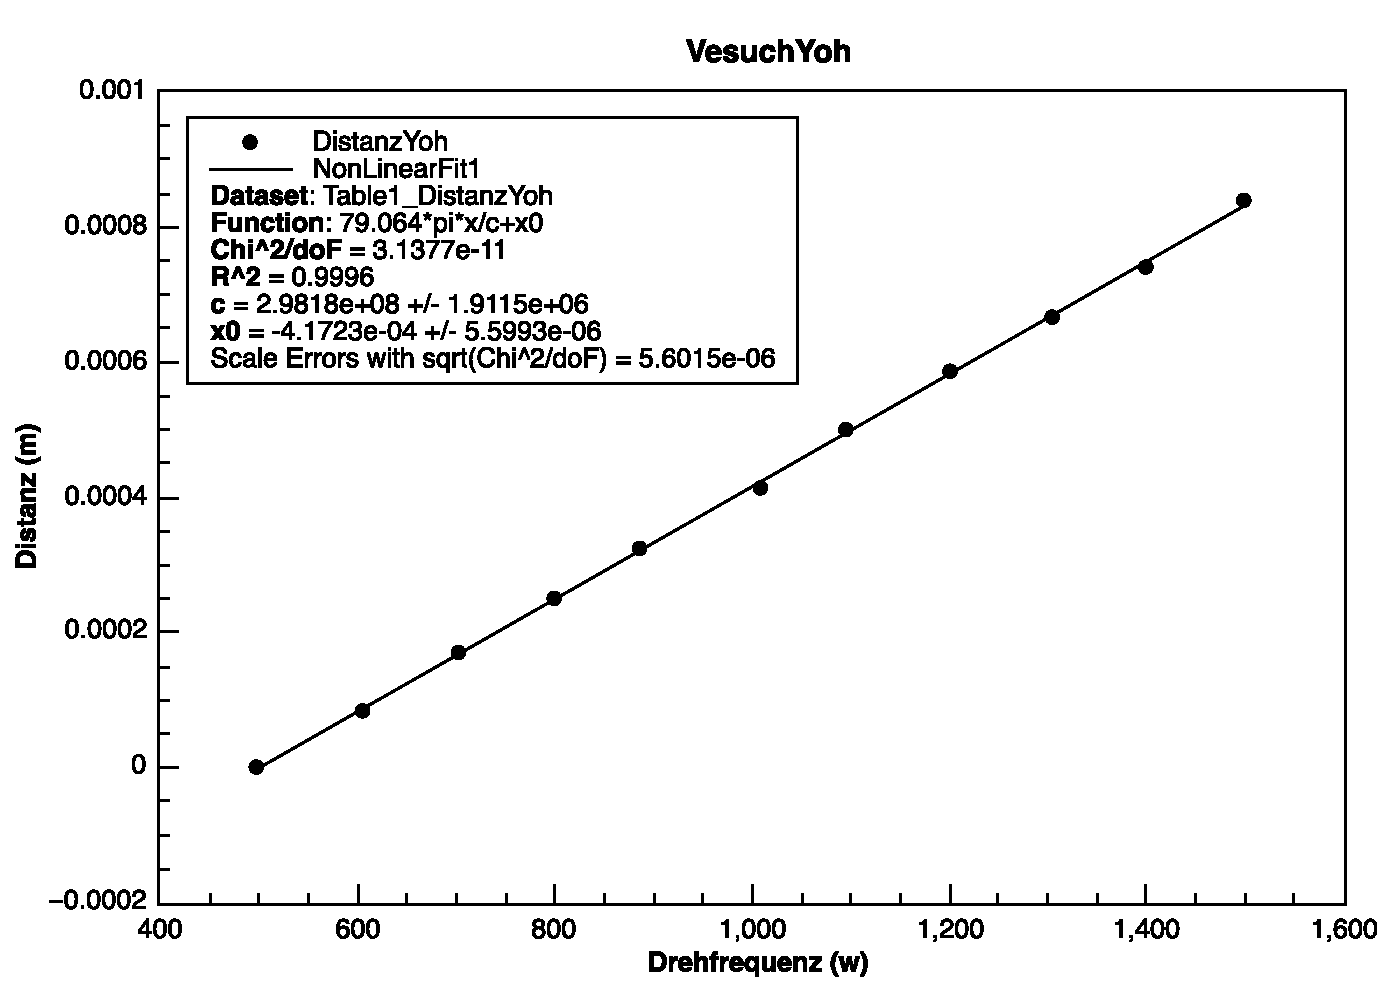
\includegraphics[width=.8\textwidth]{images/w-x-yohannes.pdf}
    \caption{XY-Scatter Plot von $\omega$ und $x$, gemessen von Yohannes Measho}
    \label{fig:w-x-yohannes}
\end{figure}

